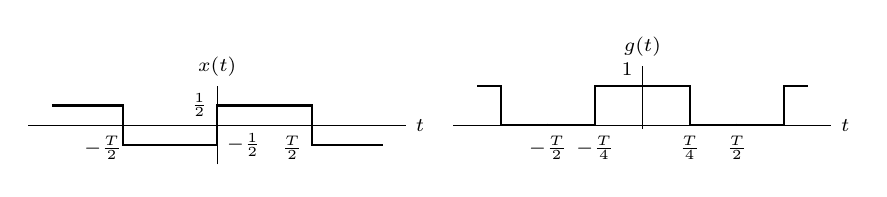
\begin{tikzpicture}[xscale=0.6, yscale=0.5]
	\begin{scope}
		\draw (-4,0) -- (4,0) node [anchor=west] {\scriptsize $t$};
		\draw (0,-1) -- (0,1) node [anchor=south] {\scriptsize $x(t)$};	
		\draw[thick] (-3.5, 0.5) -| ++(1.5, -1) -| ++(2, 1) -| ++(2, -1) -- ++(1.5, 0);
		\foreach \x/\y in {-2/{-\frac{T}{2}},  2/{\frac{T}{2}}}
		{
			\draw (\x, 1pt) -- ++(0, -2pt) node [anchor=north, xshift=-0.25cm] {\scriptsize $\y$};
		}
		\node at (0, 0.5)  [anchor=east] {\scriptsize $\frac{1}{2}$};
		\node at (0, -0.5)  [anchor=west] {\scriptsize $-\frac{1}{2}$};
	\end{scope}
	\begin{scope}[xshift=9cm]
		\draw (-4,0) -- (4,0) node [anchor=west] {\scriptsize $t$};
		\draw (0,-0.1) -- (0,1.5) node [anchor=south] {\scriptsize $g(t)$};	
		
		\draw[thick] (-3.5, 1) -| ++(0.5, -1) -| ++(2, 1) -| ++(2, -1) -| ++(2, 1) -- ++(0.5,0);
		
		\foreach \x/\y in {-2/{-\frac{T}{2}}, -1/{-\frac{T}{4}},1/{\frac{T}{4}}, 2/{\frac{T}{2}}}
		{
			\draw (\x, 1pt) -- ++(0, -2pt) node [anchor=north] {\scriptsize $\y$};
		}
		\node at (0, 1)  [anchor=south east] {\scriptsize $1$};
	\end{scope}	
\end{tikzpicture}
